\subsubsection{UC11.2 - Visualizzazione lista funzioni}
\begin{figure}[H]
	\centering
	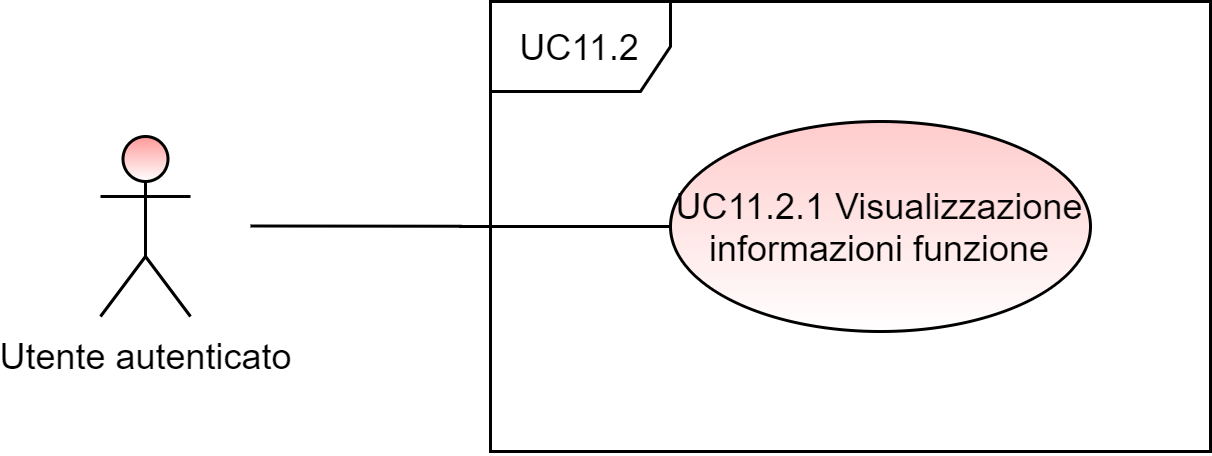
\includegraphics[scale=\ucs]{./res/img/UC11-2.png}
	\caption {UC11.2 - Visualizzazione lista funzioni}
\end{figure}
\begin{itemize}
	\item \textbf{Attori primari:} \ua{};
	\item \textbf{Descrizione:} viene visualizzata la lista ritornata dal comando \texttt{search};
	\item \textbf{Scenario principale:} viene visualizzata una lista di tutte le funzioni che nel nome contengono il termine di ricerca specificato;
	\item \textbf{Estensioni:} 
	\begin{itemize}
		\item \textbf{UC11.3:} non viene trovata alcuna funzione il cui nome contiene il termine di ricerca. Viene di conseguenza visualizzato un messaggio di avviso;
	\end{itemize}
	\item \textbf{Precondizione:} l’utente ha inserito ed eseguito correttamente il comando \search{};
	\item \textbf{Postcondizione:} la CLI\ped{\textit{G}} riporta la lista di funzioni ritornata dal comando \search{}.
\end{itemize}